
\documentclass{article}

% packages:
\usepackage{latexsym}
\usepackage{graphicx}
\usepackage{mathptmx}
\usepackage{amsmath}
\usepackage{amsfonts}
\usepackage{amssymb}
\usepackage{amsbsy}
\usepackage{amsthm}
\usepackage{listings}
\usepackage{bm}
\usepackage[section]{placeins}
\usepackage{float}

% hyperlinks:
\usepackage[pdftex,colorlinks=true,urlcolor=blue,citecolor=black,anchorcolor=black,linkcolor=black,bookmarks=false]{hyperref}

% hyphenation rules:
\usepackage{hyphenat}
\hyphenation{op-tical networks semi-conduc-tor}

% theorems:
\newtheoremstyle{scsthe}% hnamei
{8pt}% hSpace abovei
{8pt}% hSpace belowi
{\it}% hBody fonti
{}% hIndent amounti1
{\bf}% hTheorem head fontbf
{.}% hPunctuation after theorem headi
{.5em}% hSpace after theorem headi2
{}% hTheorem head spec (can be left empty, meaning `normal')i

\theoremstyle{scsthe}
\newtheorem{theorem}{Theorem}
\renewcommand{\thetheorem}{\arabic{theorem}}
\newtheorem{corollary}[theorem]{Corollary}
\renewcommand{\thecorollary}{\arabic{corollary}}
\newtheorem{definition}{Definition}
\renewcommand{\thedefinition}{\arabic{definition}}


\begin{document}


% conference:
\def\SCSconferenceacro{}
\def\SCSpublicationyear{}
\def\SCSconferencedates{}
\def\SCSconferencevenue{}

\graphicspath{{images/}{../images/}}

\title{Application of the Quantized DEVS modeling in Synchronous Machine}

% authors:
\author{
\\
}

\maketitle

\section*{Abstract}
The combination of two simulation methods -- latency Insertion Method(LIM) and Linear Implicit Quantized State Systems(LIQSS) method – provides a powerful new approach for analyzing the dynamics of network that obey energy conservation laws. For a reference system composed of 7th order Synchronous machine, and for state quantization of 0.01 percent, the method yields accuracy within 0.4 percent of that achievable with a conventional state-space solution, but using only 10percent of the number of computing cycles. The required number of compute cycles increases nonlinearly with decreasing quantization size, so that an optimum quantization size of 0.0001 was found.

\textbf{Keywords:} Stiff Systems, QDEVS, QSS, LIM, QDL

\section{Introduction}
\label{sec:intro}

Simulation analysis in support of power systems design is performed by well-separated modeling approaches. Changing the analyzed dynamics typically involves a re-modeling of the complete system, which is highly time consuming. This not only increases the modeling effort but given the complexity of some energy systems at the right time as well as the model resolution may be hard to identify. Moreover the stiffness of those systems –given by the very large range of time constants involved– makes the sole use of high-resolution models impractical for system-level long-time analyses. In this paper, we present the application of a simulation method based on Quantized State Systems (QSS) methods and Latency Insertion Method (LIM) that overcame some of the challenges associated with the simulation of multi-physics stiff energy conversion systems. This method is called Quantized DEVS-LIM, or simply \emph{QDL}.

Two powerful aspect of the QDL method are : 1) The system component models can be updated asynchronously which means models are refreshed on a component-by-component and event-by-event basis, only when required by internal change of state or by change of quantized external state of a relevant nearby component. This is an inherent benefit of this method that may result in faster calculation of states of the components and hence decrease the simulation time. 2) During long periods of steady state operation, no state updates are needed. We hypothesize that these characteristics of the method will enable us swapping the low order and high order of the models in the middle of the simulation which are often impossible for other simulators. They can either run low or high order simulation and in each case the model has to be modified and run from the start and calculate all the states from the beginning which is both time consuming and inefficient. Often we want to use the pre-run result and rerun the system with a higher or lower order subsystem injected to our current system and get the result from that section only, something that has not been possible before. 

However, QDL can use the same model and branch out only the part of the system which is of interest and explore it in more detail. “Fast-moving” and “Slow-moving” subsystem of a power distribution system will have different update rates so that slow-moving subsystem of the system will isolate fast and low-amplitude variations within those subsystems.QDL is able to simultaneously simulate different subsystems in the same simulation with varying levels of detail. For example, in case of our reference system- 7th order synchronous machine, you can continue using the same model choosing different quanta- a value which will be explained later- to do low order and high order study of the machine . This paper aims to report the benefits of the LIQSS method for simulating systems that obey the law of conservation of energy over traditional simulation methods like State Space and to do so we present the results of simulating a 7th order non linear synchronous machine consisting of both fast and slow components and show how comparable the results are compared to state space model and how QSS method is able to simulate this non linearity to derive the point. In particular, the machine model is divided into high order electrical section with slow dynamics and low order mechanical section with fast dynamics.Using QDL enables this kind of simulation more efficiently as one does not have to recreate the whole model and rerun it every time. 

Furthermore, we will report the error calculation which is the difference between state space results vs QDL results and show how states' quanta affect the states' accuracies to simulate the system in a 40-second time interval. Particularly, Using a family of plots of quantum equal to 10e-4, we will report the trajectory of states in QDL and compare it to state space results. Knowing the internal interactions in QSS method, we predict that QSS will take more time in simulating the system as we decrease the quantum size but on the other hand, the accuracy will improve hence the error decreases.

\section{Model}

The equivalent circuit on which the performance of the QSS method is studied is shown in \autoref{fig:7thOrderModelSynch}.This is a 7th order and the most complex model of the synchronous machine ignoring air gap higher harmonics, parameter changing because of external condition (such is temperature), stator and rotor windings skin effect, stator windings asymmetry, nonlinearity in iron magnetic characteristics and iron losses.Since at steady state the machine quantities are dc values the model of the system is formulated in dq in rotor reference frame so QSS does not have to update the system as in 3phase systems.This system is chosen as it has good range of speed of states where fast dynamics -low order sub-model - interact with slow dynamics-high order sub-model. Two versions of the system model were developed. One using the QDL method and the other one assembled in state space area to serve as the simulation reference. 

Both systems produce comparable prediction of the system's performance but QDL has the advantage of using the baseline model by dropping several different models of a subsystem without having to remodel the whole system from scratch, an important advantage that other simulators miss. QDL implementation of the system is written in Python language due to its simplicity and also object oriented ability so we can represent the atomic components as objects.The source code for this work written in python language with the Matlab schematic and the state space simulation files can be found at the URL \href{https://github.com/UofSC-QDEVS/shipsys} {https://github.com/UofSC-QDEVS/shipsys}.

\begin{figure}[H]
    \centering
    \includegraphics[width=0.75\textwidth]{7thOrderModelSynch.PNG}
    \caption{7th Order model of Synchronous Machine}
    \label{fig:7thOrderModelSynch}
\end{figure}
This model is represented using the differential equations. 
\begin{equation} \label{eq:lim_dependent_branch}
{\mathbf \psi}_{s} = -{\mathbf L}_{s} {\mathbf i}_{s}+{\mathbf L}_{sr} {\mathbf i}_{r}
\end{equation}

\begin{equation} \label{eq:lim_dependent_branch}
{\mathbf \psi}_{r} = -{\mathbf L}^T_{sr} {\mathbf i}_{s}+{\mathbf L}_{r} {\mathbf i}_{r}
\end{equation}

\begin{equation} \label{eq:lim_dependent_branch}
m_{e} = \psi_{d} i_{q}-\psi_{q} i_{d}
\end{equation}
\begin{equation}  \label{eq:sync1}
u_f = \nu_f + \Delta \nu_f = \nu_f + L_l \frac{d}{dt} i_f
\end{equation}


\begin{equation}  \label{eq:sync2}
\frac{d}{dt} \psi^r_d = u^r_d - L_l \frac{d}{dt} i^r_d + \omega_m L_l i^r_q - R_s i^r_d + \omega_m \psi^r_q
\end{equation}


\begin{equation}  \label{eq:sync3}
\frac{d}{dt} \psi^r_q = u^r_q - L_l \frac{d}{dt} i^r_q - \omega_m L_l i^r_d - R_s i^r_q + \omega_m \psi^r_d
\end{equation}


\begin{equation} \label{eq:sync4}
\begin{bmatrix}
\psi_d \\
\psi_F \\
\psi_D
\end{bmatrix}
= 
\begin{bmatrix}
L_d + L_l  &  M_F        &  M_D     \\
M_F        &  L^{'}_{F}  &  M_{FD}  \\
M_D        &  M_{FD}     &  L^{'}_D  
\end{bmatrix}
\begin{bmatrix}
i^r_d \\
i_F   \\
i_D   
\end{bmatrix}
\end{equation}

\begin{equation} \label{eq:sync5}
\begin{bmatrix}
\psi_q \\
\psi_Q
\end{bmatrix}
= 
\begin{bmatrix}
L_q + L_l  &  M_Q       \\   
M_Q        &  L^{'}_{Q}
\end{bmatrix}
\begin{bmatrix}
i^r_q \\
i_Q   
\end{bmatrix}
\end{equation}






Although our goal is not to introduce how the internal of a synchronous machine works, defining some setup system is necessary. The machine starts from the no-load condition. With no power delivered, all derivatives and stator currents are null. The only flow inside the system is the direct armature supported by the excitation current. The voltage generated acts only on the quadrature axis. The mechanical torque initially zero, has a ramping up to 25 percent of the nominal drive torque. In the first 15 seconds the machine is not loaded. It is only after that the machine starts to provide drive torque according to a linear law that stops 5 seconds after the trigger. The voltage must be regulated by means of a regulator which receives the error determined by the difference between a reference voltage signal of the machine and the actual voltage at the terminals. This error is used to correct the excitation. Furthermore, the model includes a filter to attenuate high frequency oscillations.

In the following sections, the background on the QDEVS-based Linear-Implicit Quantized State System (LIQSS) and the LIM modeling approach will be provided. Finally, the results are presented comparing the state space simulation to QDL approach. 

\section{Background}

Traditional approaches to simulate a system are based on time discretization like Euler forward and backward. While traditional discrete-time simulators divide the simulation time into time spaced intervals at which a result is calculated, quantized state systems (QSS) methods are the dual of the time integration approaches and are based on state quantization which divide the solution domain into spaced quantized values at which a time is calculated. At these times an event is generated and this is why this method is called Event-Driven approach to solve the simulation. In general, a quantized simulation approach allows the user to choose the resolution of the output, a value normally called a quantum, which results in identifying the time of the events for the values of interest. Choosing the quantum as small or large has different results and is inversely proportional to the accuracy of the output value. In comparison with a small quantum, a larger quantum will make the system update less frequently, especially as it reaches dc steady-state. This can be beneficial because a larger quantum will result in faster simulation runs obviously at the price of reduced accuracy. Most importantly, if the system is in a quasi-steady-state the simulation only updates during the transition from one steady-state to another, with frequent updates performed during the transition. A generic QSS model can be conveniently formalized using the Discrete Event System Specification (DEVS) formalism. In the following we go over the description of this approach briefly. For more thorough explanations one can refer to  \cite{cellier2006continuous}. Previous attempts at implementing QDEVS-LIM approach can be found at  \cite{benigni1}."Joe and Dr.Dougal" paper describes the theory of a new simulation method applied to electric power systems.

\subsection{Latency Insertion Method} 

The Latency Insersion Method, as described in \cite{schutt1}, uses system latency so as to permit complete decoupling of the system equations by exploiting existing latency, or inserting small, fictitious latency at nodes and branches where no significant physical latency exists which makes sense since practically speaking these latency exist in parts of the system but in most simulations, researches ignore them for simplicity of their models. The method enforces  Kirchoff's Voltage Law (KVL) and Kirchoff's Current Law (KCL) on the network. LIM is thus based on the solution of a generic branch type and of a generic node type. \autoref{fig:lim_dependent_node} and \autoref{fig:lim_dependent_branch} respectively show how a generic node and a generic branch are represented using LIM approach and this approach has been followed through out the whole modeling of our system. 


\begin{figure}[htb]
    \centering
    \includegraphics[width=0.35\textwidth]{lim_dependent_node.png}
    \caption{Generic LIM node with dependent sources.}
    \label{fig:lim_dependent_node}
\end{figure}

\begin{figure}[htb]
    \centering
    \includegraphics[width=0.35\textwidth]{lim_dependent_branch.png}
    \caption{Generic LIM branch with dependent sources.}
     \label{fig:lim_dependent_branch}
\end{figure}

\section{QSS IMPLEMENTATION}
In the following family of plots, the results of the QSS vs State Space (SS) using Euler as the reference frame method are reported. In each plot, the trajectory of the value of interest is reported using both QSS and SS in addition to the number of the updates the system has gone through to generate that value which depends heavily on the quantum chosen. The quantum chosen for these plots is 10e-4 which is a pretty reasonable value in QSS method. The plots show that QSS is very able to follow the path of SS. 

It is worth noting that one advantage of QSS method over equally time discretization methods is that in steady state condition, the system does not experience many updates and the number drops heavily. For example, between 15 sec to 35 seconds that the dynamics of the system is changing, the slope of the red line representing the cumulative number of updates is way more than the section between 35 sec to 40 sec where the red line sloped down since we are in steady state condition. This aspect of the QSS method causes the system to be simulated very fast during steady state condition. 
 \begin{figure}[H] 
    \FloatBarrier
    \centering
    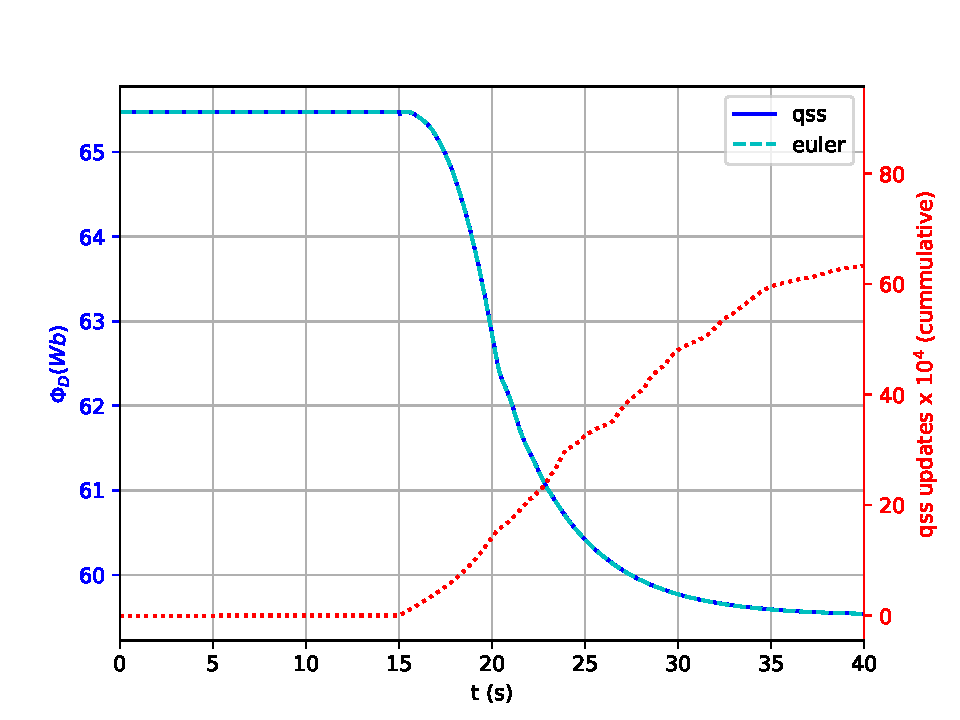
\includegraphics[width=0.50\textwidth]{fD_full_dq_1e-4.pdf}
    \caption{Results of fictitious phi D}
    \label{fig:fD}
\end{figure}

Furthermore, the cumulative number of updates depends on the quantum chosen. In \autoref{fig:fD} for example, the quantum chosen for this value is plotted in 2 ways. One with q1=1e-4 and with q2=1e-5. The latter quantum being smaller causes the system to go through more updates and hence the finishing point of the yellow line is higher than the red line with quantum equal to 1e-4. We could not find a linear relationship between the surge in the number of updates and how much the quantum size is reduced or got bigger. 

The following graph is an example of the asynchronous behavior of the QDL method. One might think that all the atoms of the system go through the same number of updates but the following graph refutes that statement. The atoms got updates only when their internal state changes as the time advance is up or by external updates which happen due to change of quantized state of neighbor nodes of that atom. Furthermore, \autoref{fig:fdr} shows how closely QDL can track both the electromechanical behavior from 20 sec to 25 sec and the mechanical behavior of the system. The electrical behavior of the system is shown in \autoref{fig:qss ripples} where zooming the plots shows the ripples existing in QDL method. 

 \begin{figure}[H]
 \FloatBarrier
    \centering
    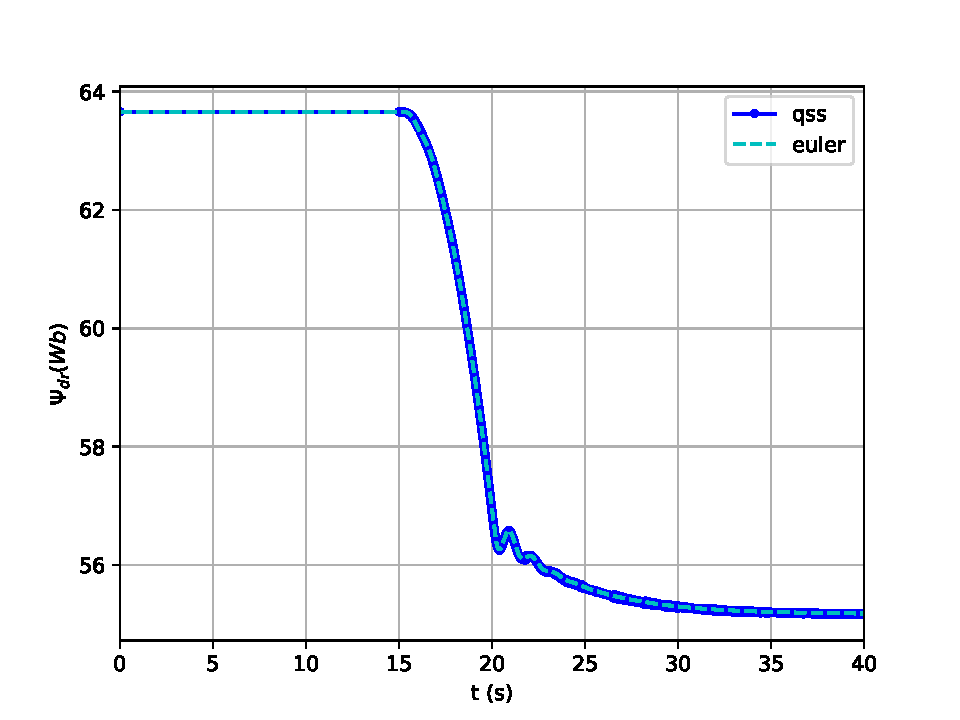
\includegraphics[width=0.50\textwidth]{fdr_full_dq_1e-4.pdf}
    \caption{Results of rotor d-axis flux}
    \label{fig:fdr}
\end{figure}

 \begin{figure}[H]
 \FloatBarrier
    \centering
    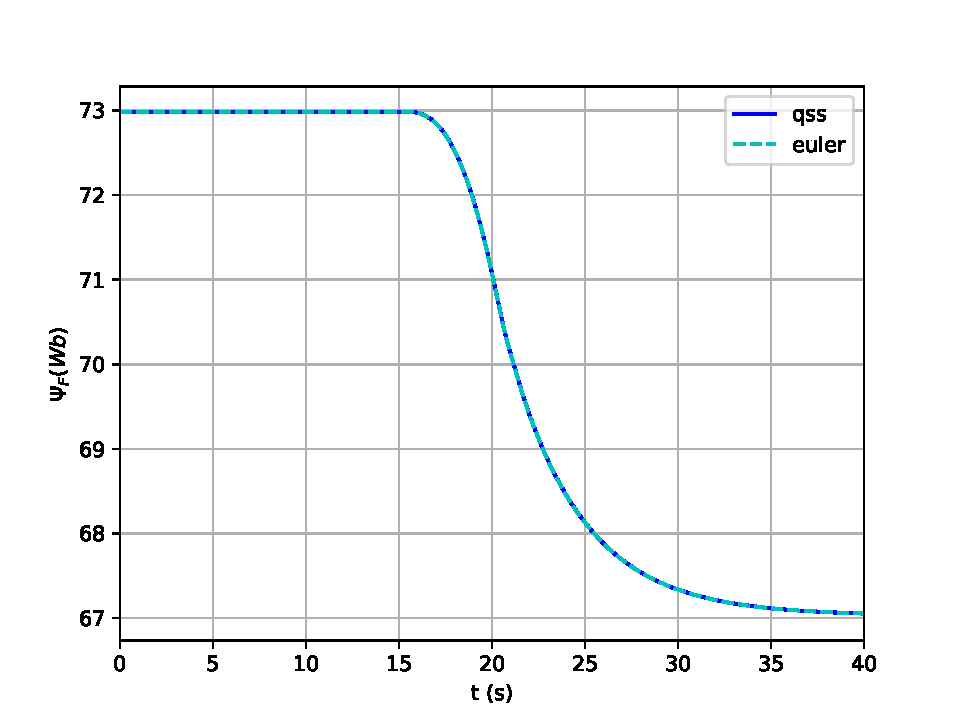
\includegraphics[width=0.50\textwidth]{fF_full_dq_1e-4.pdf}
    \caption{Results of field flux}
    \label{fig:filed current flux}
\end{figure}


 \begin{figure}[H]
 \FloatBarrier
    \centering
    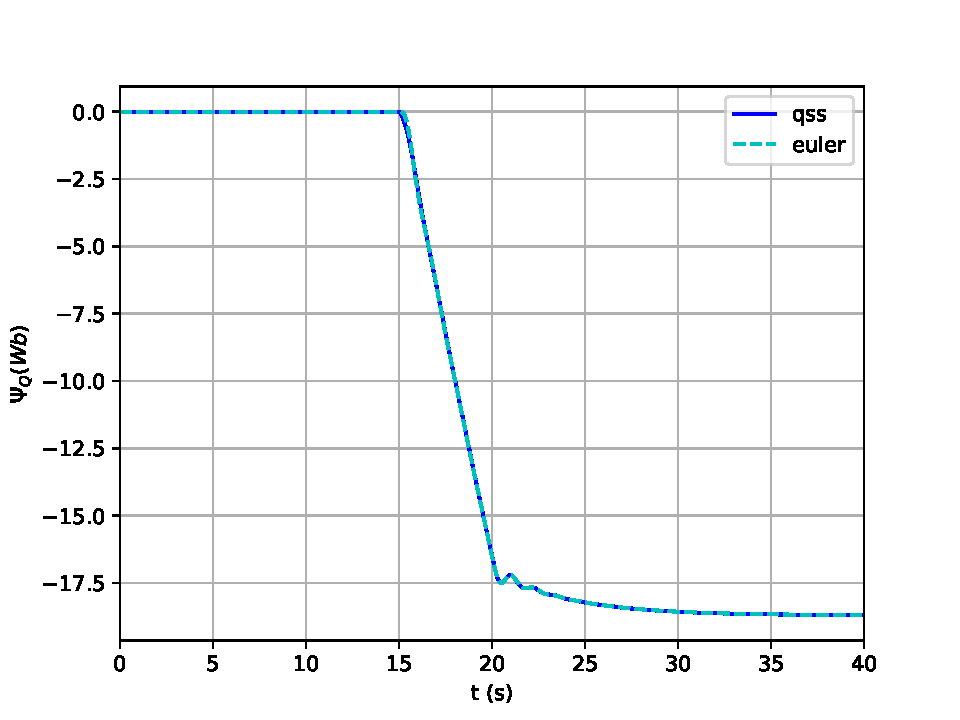
\includegraphics[width=0.50\textwidth]{fQ_full_dq_1e-4.pdf}
    \caption{Results of fictitious Q}
    \label{fig:fQ}
\end{figure}

 \begin{figure}[H]
 \FloatBarrier
    \centering
    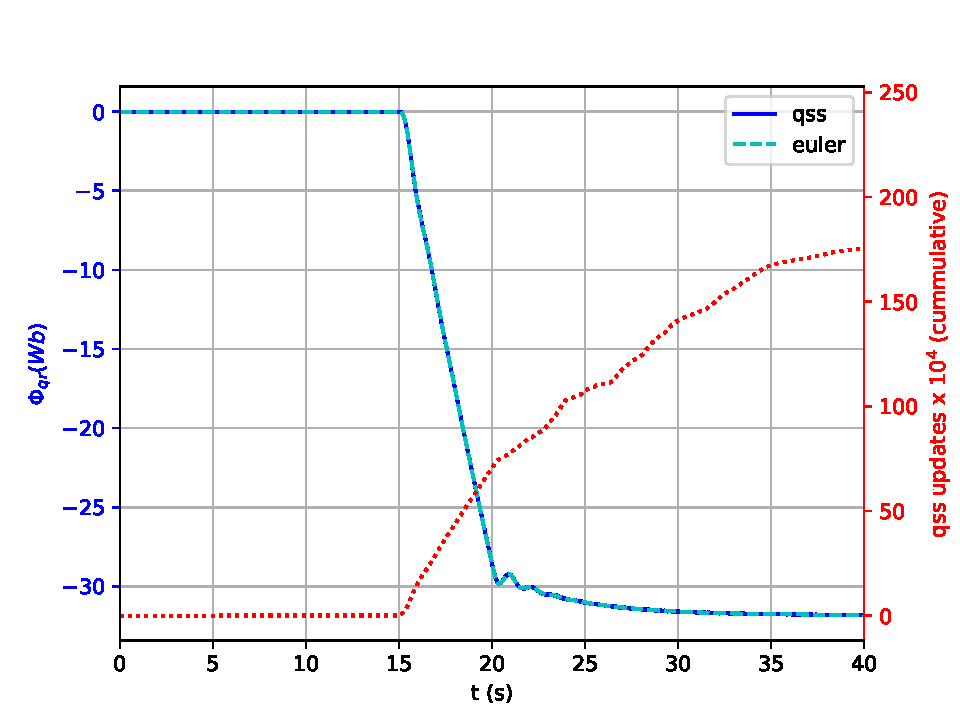
\includegraphics[width=0.50\textwidth]{fqr_full_dq_1e-4.pdf}
    \caption{Results of rotor q-axis flux}
    \label{fig:fqr}
\end{figure}

Before the machine is loaded, the quantities only are present on the direct axis. This is because the machine is not generating any power so currents are only due to excitation on the direct axis. When the machine is loaded the flows decreases. The minus sign in both id and iq represent the the system is consuming power. 

Results for rotor angel

The trend of the mechanical variables shows how the machine actually takes charge after 15 seconds, after the insertion of the driving torque, the delta angle increases and the speed temporarily increases. After 20 seconds, when the power supplied to the machine becomes constant, everything stabilizes at steady state values.

 \begin{figure}[H]
 \FloatBarrier
    \centering
    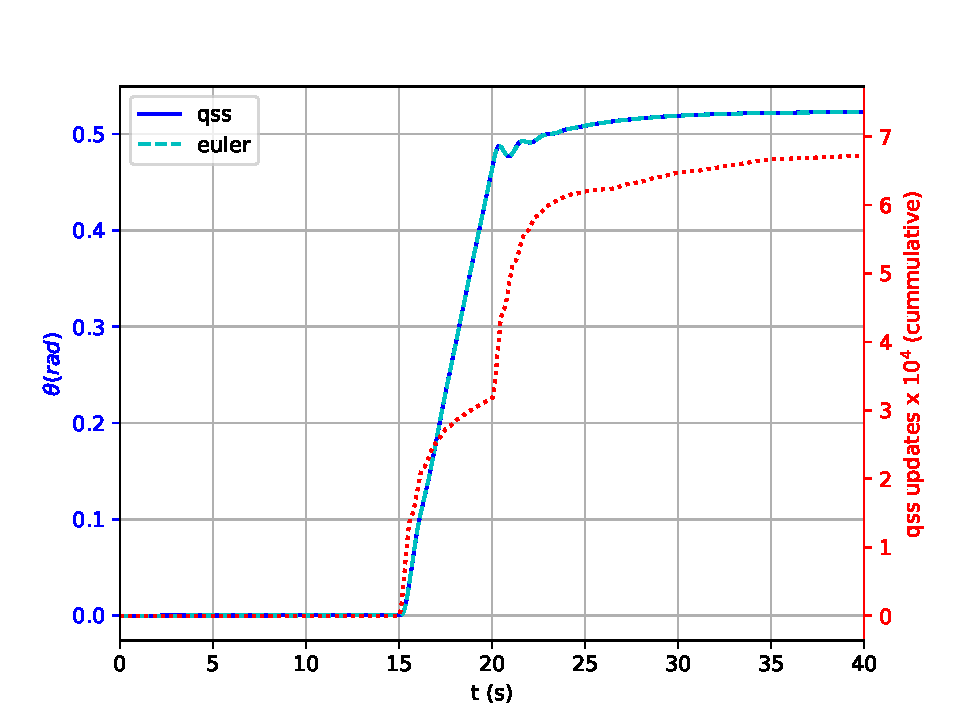
\includegraphics[width=0.50\textwidth]{theta _full_dq_1e-4.pdf}
    \caption{Results of theta}
    \label{fig:tehta}
\end{figure}
The trajectory of the mechanical variables show after 15 seconds when the driving torque is inserted, the delta angle increases and the speed temporarily increases. 5 Seconds later when the power supplied to the machine becomes constant, everything stabilizes at steady state values. 
Before the 15 seconds machine is not delivering any active power as it is expected and only supply reactive power since it is in the state of over excitation.
The trajectory of theta is particularly interesting since the qss updates show that the value between 15 to 20 seconds tries to reach the steady state but the dynamics of the systems changes and it goes through another round of updates where at almost 23 seconds the updates start to level off and reaches the final steady state. 

 \begin{figure}[H]
 \FloatBarrier
    \centering
    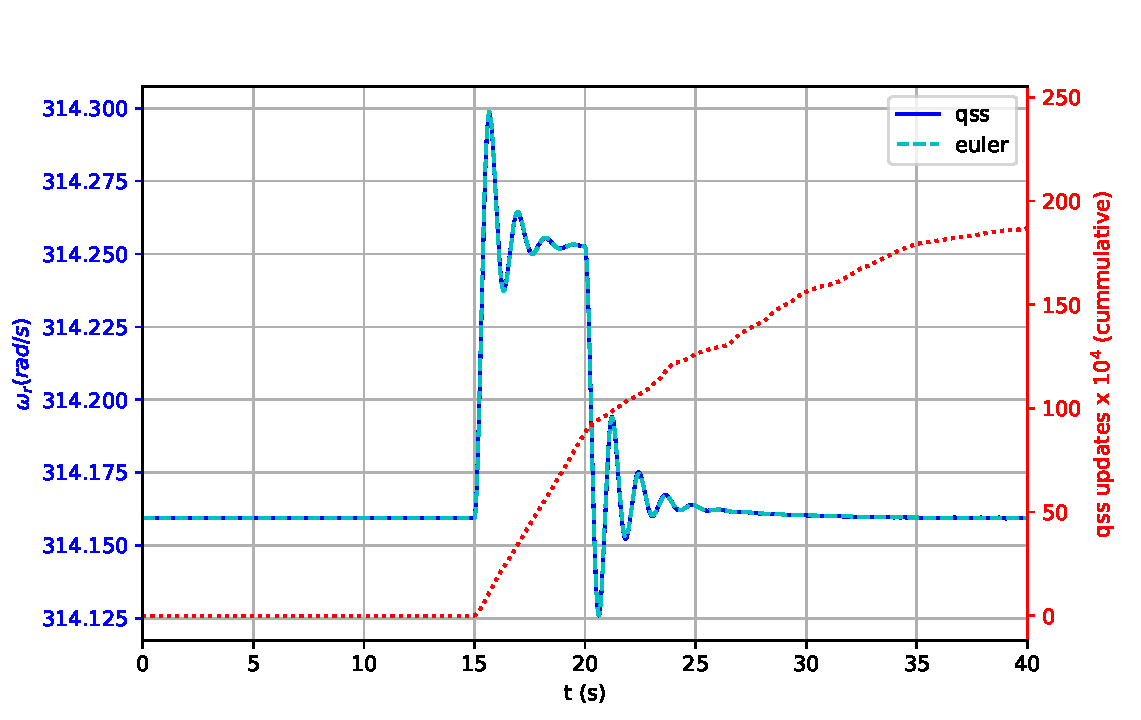
\includegraphics[width=0.50\textwidth]{wr_full_dq_1e-4.pdf}
    \caption{Results of rotor speed}
    \label{fig:wr}
\end{figure}

In \autoref{fig:id} and \autoref{fig:vd} the number of cumulative updates are not shown since these values are the derived values from the fluxes. They show QDL not only can track the direct values, but also is able to track the derived values which are the same as the differential equations.  

 \begin{figure}[H]
 \FloatBarrier
    \centering
    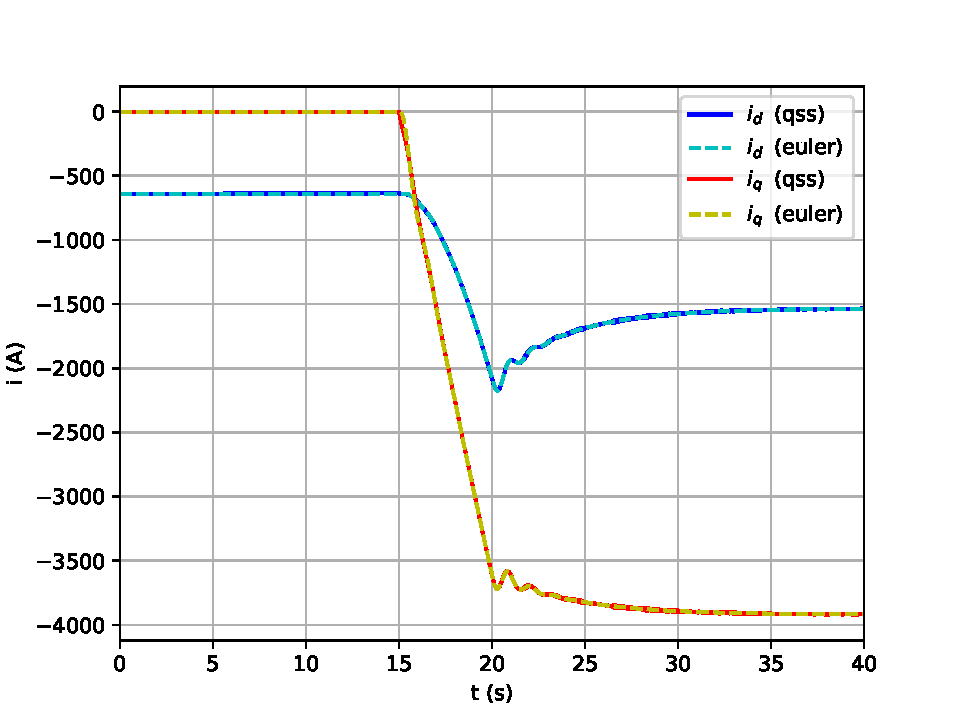
\includegraphics[width=0.50\textwidth]{currents_full_dq_1e-4.pdf}
    \caption{rotor id and iq}
    \label{fig:id}
\end{figure}

 \begin{figure}[H]
 \FloatBarrier
    \centering
    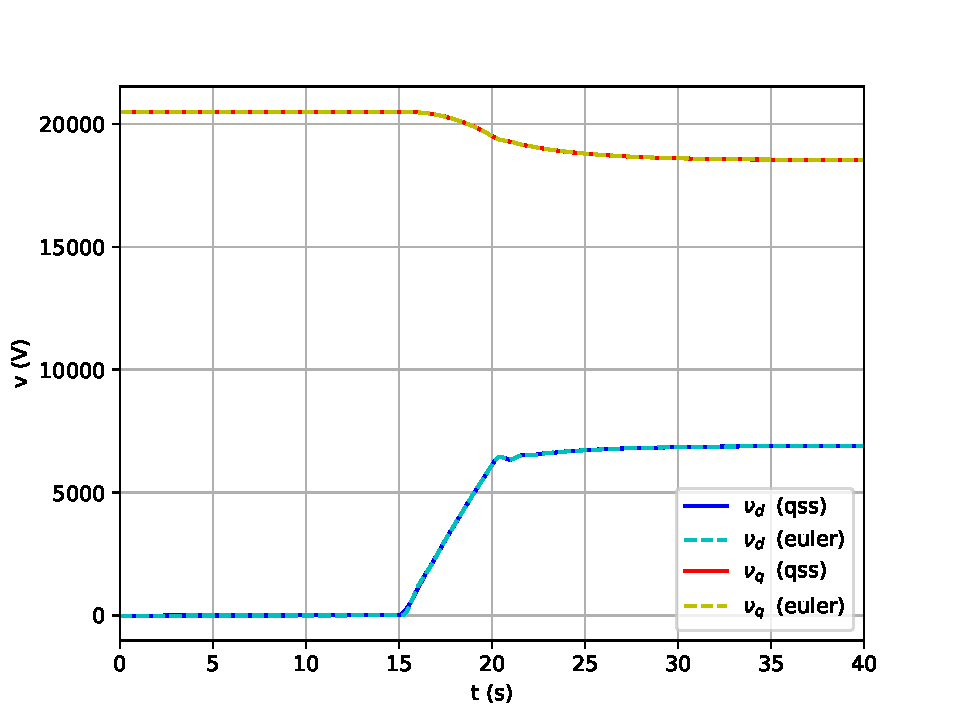
\includegraphics[width=0.50\textwidth]{volts_full_dq_1e-4.pdf}
    \caption{d-axis voltage and q-axis voltage}
    \label{fig:vd}
\end{figure}



\subsection{Accuracy and Error analysis}
In short the error is the difference of state space results compared to QDL results and is calculated according to 
\begin{equation} \label{eq:Normalized Relative RootMean Square Error}
error= \frac{\sqrt{sum((y-q)^2)/N}} {max(y)-min(y)}
\end{equation}
The nominator is the root square of sum of all squared values of actual states(y) minus the quantized states(q) divided by total number of states(N). The denominator tries to normalize the error and is the maximum of the state value minus the minimum of the state value for that particular variable.

In \autoref{fig:relativeError}, the error for fdr over 0.5 second is shown. The quantum is ranging from a very low value 10e-6 to 10e-2. Clearly bigger quantum produces bigger error and vice versa. The 3 quantum values almost start from zero error until the system dynamics changes and so the number of updates starts to grow where the 3 quanta starts to produce different errors. However, one might decide to choose a big quantum like 10e-2 for the whole system if 1 percent of error (in our case) is tolerable and the speed is of essence in these applications. However, a small quantization size causes a large model update rate that does improve the simulation accuracy as the error amplitude decrease respectively. Unfortunately, we could not find a linear relationship between the amount of increase in quantum value and the amount of increase in the error amplitude. But one thing for sure happens is that larger quantum results in less update rates and higher error amplitude compared to smaller quantum values with more update rates and lower error amplitude.

\begin{figure}[H]
 \FloatBarrier
    \centering
    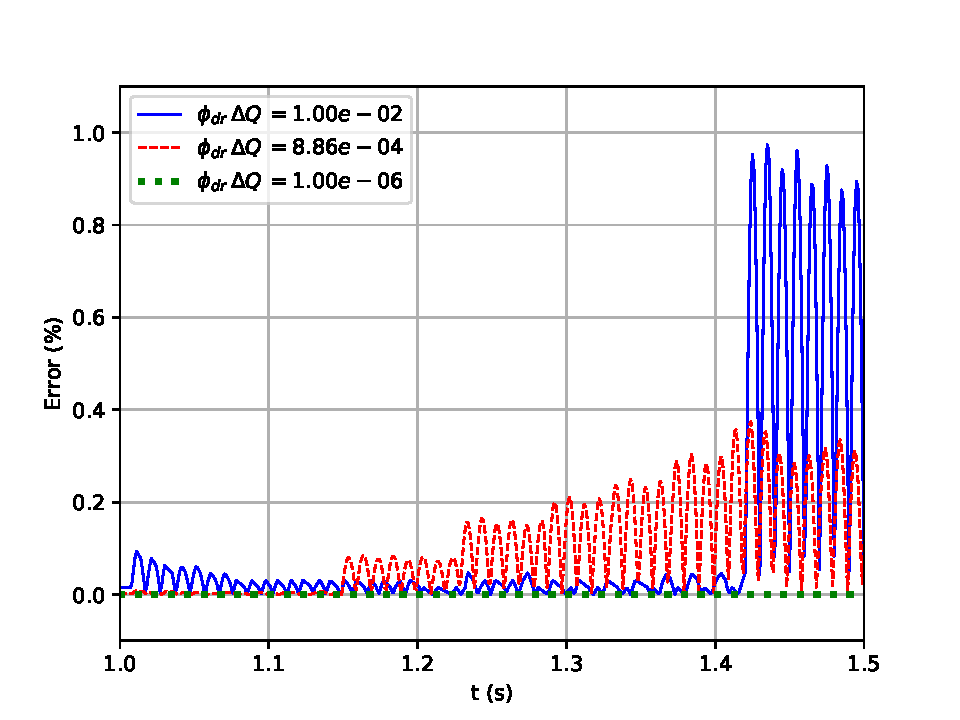
\includegraphics[width=0.50\textwidth]{fdr_error_over_time_rev1.pdf}
    \caption{Results of error}
    \label{fig:relativeError}
\end{figure}

In \autoref{fig:maxerror} the maximum error of each atom is plotted on a logarithmic scale against number of updates for 1 second of transient time. The quanta are changing from 10e-6 to 10e-2 showing how error is affected by the quantum value. From 10e-6 to 10e-5 the error seems to be near zero with a very minute changes. So it seems unnecessary to choose such a low quantum as it only makes the simulation run longer than needed. The sweet spot here is a quantum in the range of 10e-5 to 10e-4 where the error starts to jump. One might observe once the error increases the total number of updates decreases and this completely makes sense since as you choose a bigger quantum, the number of updates reduces at the expense of a jump in the error. One might choose a quantum based on these plots. 

\begin{figure}[H]
  \FloatBarrier
    \centering
    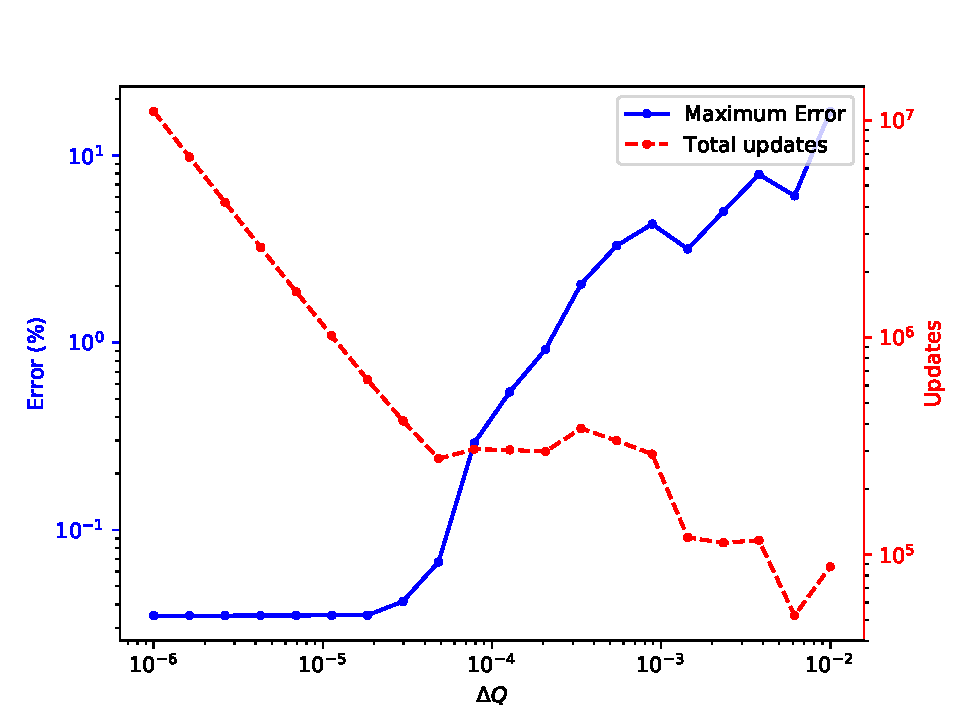
\includegraphics[width=0.50\textwidth]{error_vs_updates_rev3.pdf}
    \caption{Results of error}
    \label{fig:maxerror}
\end{figure}

As we observed previously, QDL is very able to track the state space solution but there is a caveat. While using QDL, since the updates are propagated almost simultaneously, the trajectories sometimes appear as less damped as it should be but in state space solution since there is a delay in propagating the update signals, rarely we will see these ripples.However, as the quantum values are approaching smaller values towards zero, theoretically, these ripples should disappear but once again this comes at the cost of time it takes to simulate the system. In \autoref{fig:qss ripples1}  with quantum value equal to 1e-5 and \autoref{fig:qss ripples2} with quantum value equal to 1e-4, when we zoom enough these ripples starts to bubble up. As we said, one might want to get rid of these ripples by choosing a quantum size almost near zero.
\begin{figure}[H]
  \FloatBarrier
    \centering
    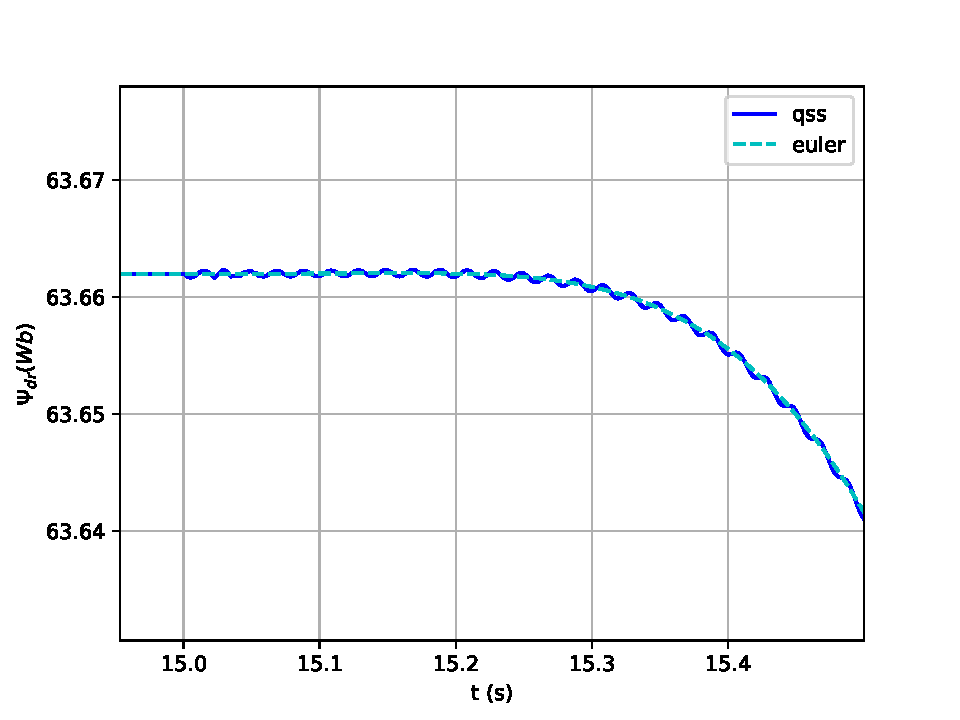
\includegraphics[width=0.50\textwidth]{fdr_ZOOM2_dq_1e-5.pdf}
    \caption{ripples in fdr with q=1e-5 }
    \label{fig:qss ripples1}
\end{figure}

\begin{figure}[H]
  \FloatBarrier
    \centering
    \includegraphics[width=0.50\textwidth]{fqr_ZOOM4_dq_1e-4 copy.pdf}
    \caption{ripples in fdr with q=1e-4}
    \label{fig:qss ripples2}
\end{figure}



\section{Conclusion}

A method for simulating a non linear synchronous machine model was presented, using the QDEVS-based formulation and the LIM modeling method. The combined method is called QDL, and is shown to be efficient in simulating the dynamics of the synchronous machine.

% references:

\bibliographystyle{scsproc}
\bibliography{references}

\end{document}
